\documentclass[a4paper,10pt]{article}
\usepackage[utf8]{inputenc}
\usepackage{graphicx}
\usepackage{hyperref}

%opening
\title{Artificial Intelligence \\ notes}
\author{Klara Malinowska}

\begin{document}

\maketitle

\tableofcontents
\newpage

\section{Welcome to AI}
\subsection{Terminology}

\paragraph{Fully/partially observable}
The environment is fully observable if what the agent can sense at any point of time is sufficient to make and optimal decision. In partially observable environment the memory of previous states is required to make an optimal decision.

\paragraph{Deterministic/stochastic}
In deterministic environment the effect of an agent actions uniquely determines the outcome. In stochastic environment - the outcome of the action have a certain level of randomness.

\paragraph{Discrete/continuous}
In discrete environment the finally actions choices and things to sense. In continuous environment there is may be unlimited amount of possible actions or things to sense.

\paragraph{Benign/adversarial}
The benign environment does not have an objective that contradicts your objective. In adversarial the environment actively observes the agent actions and counteracts with what it is trying to achieve.

\section{Problem Solving}

Complexity may come from large number of possible choices or from partial observability.

\paragraph{Definition of an problem}
The problem may be defined by a set of states and functions
\begin{enumerate}
  \item Initial state $s$
  \item Action($s$) $\rightarrow$ $a$ There may be a lot of them forming a set ${a_1, a_2, ...}$ and they may be dependent or independent on a current state
  \item Result($s,a$) $\rightarrow$ $s'$ Taking initial state and a chosen action gives us the resulting state.
  \item GoalTest($s$) $\rightarrow$ $s'$ T|F Takes a current states and checks if it is a solution. Returns boolean value.
  \item PathCost($s,a,s,a,s,...$) $\rightarrow$ $n$ Takes sequence of steps and actions and gives a cost of it as a number. Usually is an additive function of StepCosts
  \item StepCost($s,a,s'$) $\rightarrow$ $n$ Gives a cost of one action as a number.
\end{enumerate}

States space divides into explored part, frontier (which are the farthest state explored) and unexplored part.

A problem solving technology works only if the domain is:
\begin{enumerate}
 \item fully observable (we know exactly the current state)
 \item known (known set of available actions)
 \item discrete(limited amount of possible actions)
 \item deterministic (result of an action is known)
 \item static (nothing changes the space state but we)
\end{enumerate}

\subsection{Path searching}

\paragraph{Tree search vs. graph search} 

The two search algorithms differ in ``having memory'' - remembering which states are already explored. The tree algorithm does not do that, so it can go back with the explored path to the state it has already been in. The graph search remembers where it has already been and thus never goes back to the previously visited states.
\paragraph{Tree search}
\begin{verbatim}
function Tree.Search(problem)
  frontier = {[initial]}
  loop:
    if frontier is empty: return FAIL
    path = remove_choice(frontier)
    s = path.end
    if s is a goal: return path
    for a in actions:
      add [path + a -> Result(s,a)] to frontier
\end{verbatim}

\paragraph{Graph search}
\begin{verbatim}
function Tree.Search(problem)
  frontier = {[initial]}
  explored = {}
  loop:
    if frontier is empty: return FAIL
    path = remove_choice(frontier)
    s = path.end
    add s to explored
    if s is a goal: return path
    for a in actions:
      add [path + a -> Result(s,a)] to frontier 
      unless Result(s,a) in frontier + explored
\end{verbatim}

\paragraph{Breadth first search}
Always chooses the shortest (in term of steps) path to explore next. If there are paths of the same length, it chooses randomly. Is guaranteed to find the shortest (in terms of number of steps) path. Requires storage space of $2^n$ paths to store all the nodes in the frontier.

\paragraph{Uniform-cost search - cheapest first}
It chooses which path to explore next basing on the path cost. Is guaranteed to find the cheapest path, because even if it has already added the goal to the frontier, it firstly explores all the shorter paths and only when the one leading to the goal is the shortest it performs the goal check. Number of paths in the frontier is similar that in the breadth first algorithm.

\paragraph{Depth first search}
It chooses the longest path to explore first. It is not optimal - does not guarantee to find the best solution (path that reaches the goal in the minimal amount of steps). Requires storage space of $n$ to store all the nodes in the frontier.

\paragraph{Number of nodes in the frontier}
It is $2^n$ for the breadth first search and similar in the uniform-cost search. It is $n$ in the depth first search. Thus depth first search requires much less memory than the other two when we save the frontier only. However, if we save also explored space, all three algorithms need the similar amount of memory.

\paragraph{Completeness}
Algorithm is complete if it will always find the optimal path. Breadth first and uniform-cost search algorithms are complete. The depth first search algorithm is not.

\paragraph{Greedy best-first search}
It needs additional information to work, eg. estimate of the distance of the start state to the goal such as straight line distance from the state to the goal. It explores much smaller part of the states space that the uniform-cost search, and therefore shall be faster. However, it may not find the shortest path (if it requires going in the direction ``from'' the goal in some steps) - it is not complete.

\subsection{A* search}
The A* search combines the uniform-cost search and greedy best-first search in its way to determine which path to explore. It chooses the path to explore minimizing on the function h(path) which adds the path cost up to certain state as well as distance from the goal.
\begin{verbatim}
f(path) = g(path) + h(path)
g(path) = path.cost
h(path) = h(s) = current distance to the goal
\end{verbatim}

The A* algorithm will always find the lowest cost path if h(s) function is smaller than a true cost to get to the goal from a current state. It should never overestimate the cost to get to the goal, an thus is an  optimistic. Such an h is called \textbf{admissible} (it is admissible to use it to find a lowest cost path). 

\section{Probability in AI}

\subsection{Probability properties}
\begin{itemize}
\item \textbf{Complementary events} The event $A$ and its complement $\neg A$ are mutually exclusive and exhaustive.
\[p(A) = 1 \Rightarrow p(\neg A) = 1-p \]
\item \textbf{Independence of events} Two events are independent ($A\perp B$) means that the occurrence of one event makes it neither more nor less probable that the other occurs.
\[ A\perp B \Leftrightarrow P(A,B) = P(A)P(B) \]
\item \textbf{Conditional probability} is the probability that event A occurs when the sample space is limited to event B. This is read "the probability of A, given B" and denoted as $P(A\mid B)$.
\[P(A|B,C) = \frac{P(A,B,C)}{P(B,C)} \]
\[P(\neg A\mid B) = 1-P(A \mid B) \]
\item \textbf{The law of total probability}
If $A_i$ is a set of pairwise disjoint events whose union is the entire sample space, then
\[P(B) = \sum_{i} P(A \mid B_i)P(A_i) \]
\item \textbf{Bayes rule}
\[ P(A|B) = \frac{P(B|A)P(A)}{P(B)} \]
\[ P(A|B,C) = \frac{P(B|A,C)P(A)}{P(B|C)} \]
In this expression $P(A|B)$ is called \textbf{posterior} $P(B|A)$ is called \textbf{likelihood}, $P(A)$ is called \textbf{prior} and $P(B)$ is called \textbf{marginal likelihood}. 

The Bayes rule can be written differently using the law of total probability:
\[ P(A_j|B) = \frac{P(B|A_j)P(A_j)}{\sum_{i} P(A \mid B_i)P(A_i)} \]
It can be also written omitting the usage of $P(B)$ by introducing \textbf{normalizer} $\eta$ defined as
\[ \eta =(P'(A|B)+P'(\neg A|B)) \]
where
\[ P'(A|B) = P(B|A)P(A) \]
\[ P'(\neg A|B) = P(B|\neg A)P(\neg A)\]
Than the Bayes rule can be written as
\[ P(A|B) = \eta P'(A|B) \]

\item \textbf{Conditional independence} The probability of outcome of two events $T_1$ and $T_2$ is dependent of the state of the event C. Those two events are conditionally independent independent given C if
\[ P(T_2|C,T_1)=P(T_2|C) \]
That means that if we know the outcome of event $C$, the probability of outcomes of event $T_2$ does not depend of the outcome of the event $T_1$. The conditional independence of events $T_1$ and $T_2$ given the outcome of event C is denoted as:
\[T_1 \bot T_2 | C \]
\item Conditional independence does not imply the absolute independence, and absolute independence does not imply conditional independence.

\end{itemize}

\subsection{Bayes networks}

A Bayes network is a probabilistic graphical model that represents a set of random variables and their conditional dependencies via a directed acyclic graph. The nodes of the graph represent the variables, and the edges represent the conditional dependences. 

Structured Bayes networks need to store much less numerical information than an unstructured representations of probability distributions. Bayes networks are much more compact.

They are used to reason within known models, that can be described mathematically as beysesian networks.

\subsubsection{Basic types of Bayes networks}

\begin{figure}[h!]
\centering
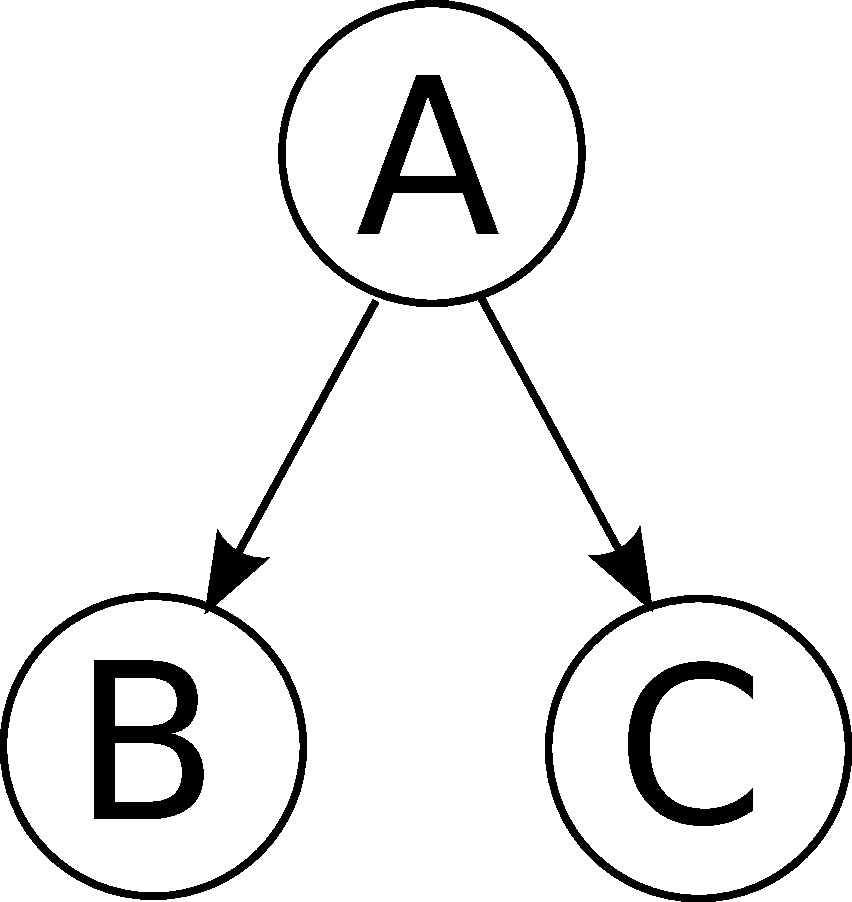
\includegraphics[height=0.2\textwidth]{Bayes1.pdf} \hspace{2em}
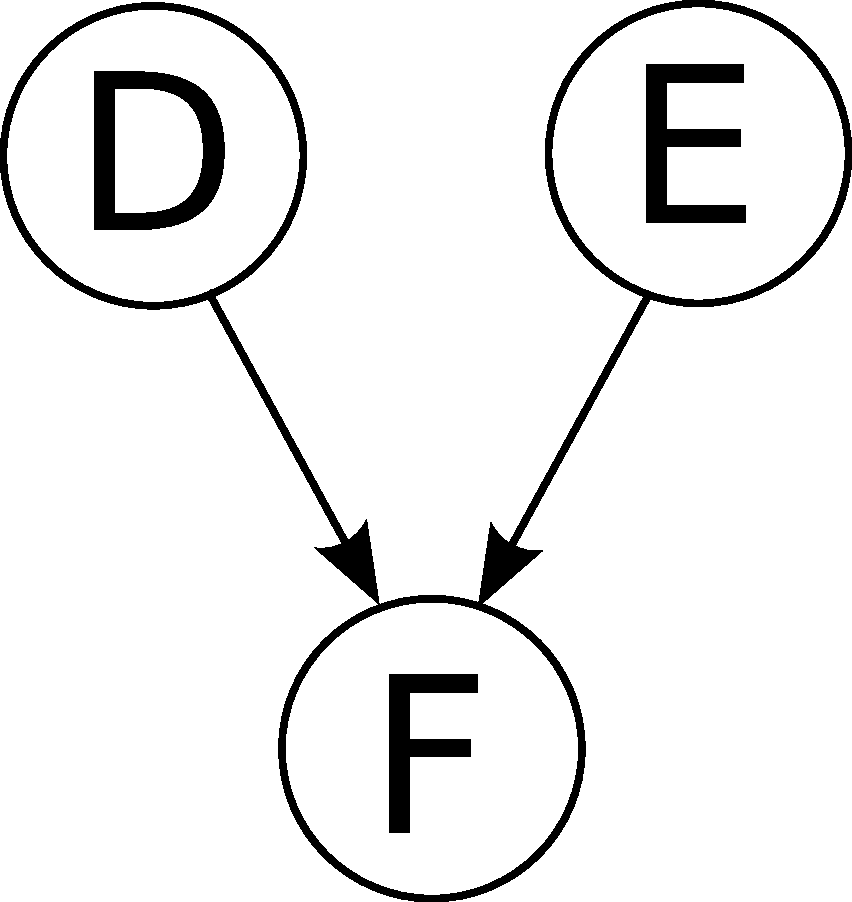
\includegraphics[height=0.2\textwidth]{Bayes2.pdf}
\end{figure}

To define the network on the left we need three values of probabilities: $P(A)$, $P(B|A)$ and $P(C|A)$. The probabilities of different values of events B and C depend on the value of the value of the event A. Thus the events B and C are dependent on event A. The events B and C conditionally independent given the value of A. However, if the value of A is not known, the events B and C are dependent on each other.

To define the network on the right we need to know $P(D)$, $P(E)$ and $P(F|D,E)$.The probability of different values of the event F is dependent on the values of the events D and E. Thus the event F is conditionally dependent on the events D and E. The events D and E are independent on each other if we don't know the value of the event F, but they are conditionally dependent given the value the event F.

\begin{figure}[h!]
\centering
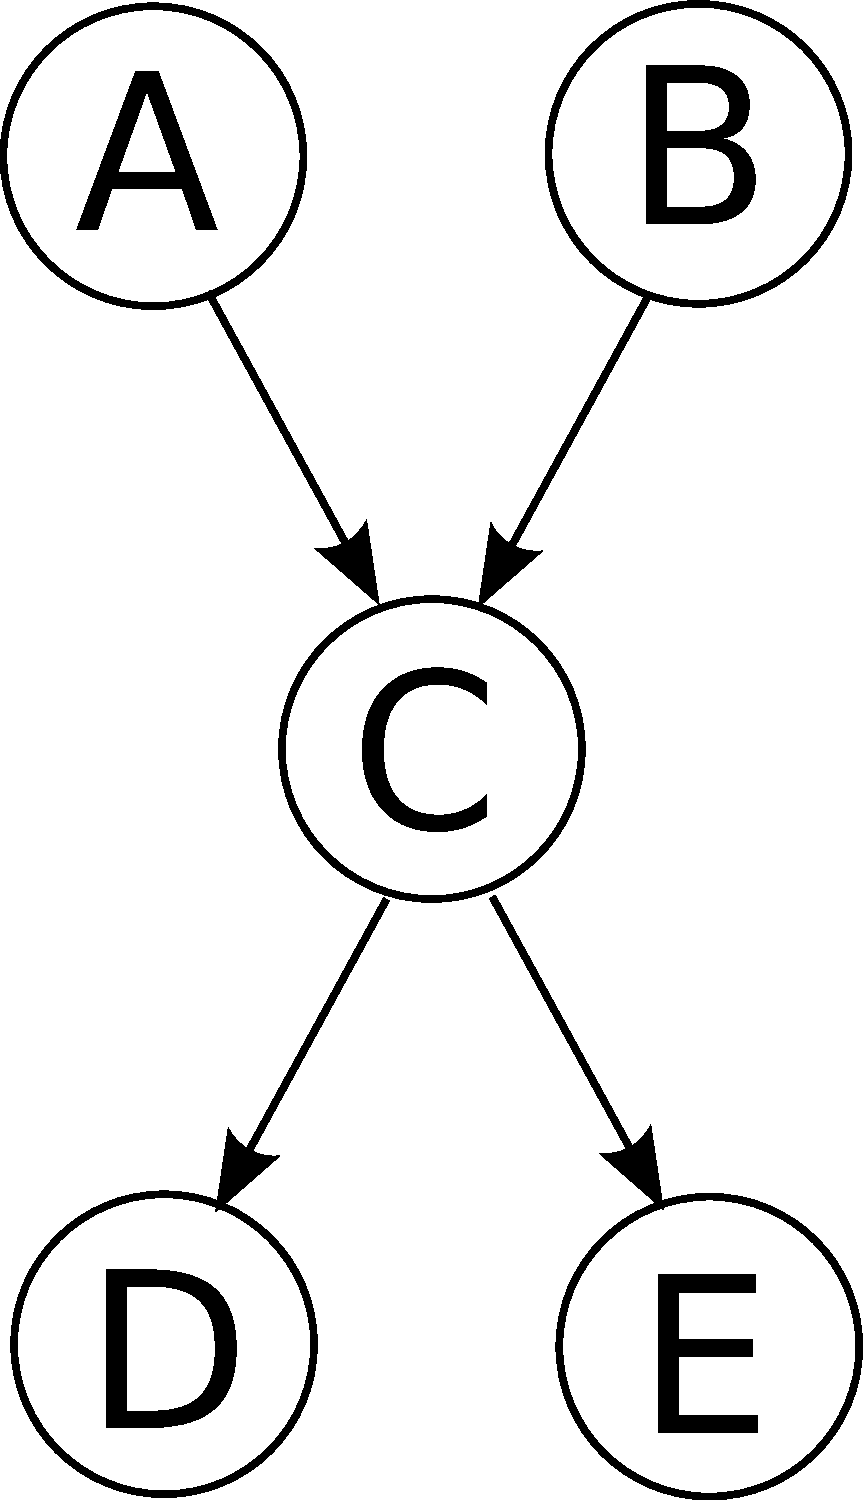
\includegraphics[height=0.3\textwidth]{Bayes3.pdf}
\end{figure}
To define such a distribution of probabilities we need to know $P(A)$ and $P(B)$, because they don't have the incoming edges, and the conditional distributions $P(C|A,B)$, $P(D|C)$ and $P(E|C)$. Thus we need 10 numerical values (in general $2^n$ values for each node with $n$ incoming edges). The joined distribution of all of the nodes in the network can be calculated as
\[ P(A,B,C,D,E) = P(A)P(B)P(C|A,B)P(D|C)P(E|C)\]

\subsubsection{D-separation}
\paragraph*{Dependent events in the Bayes networks}

\begin{figure}[h!]
\centering
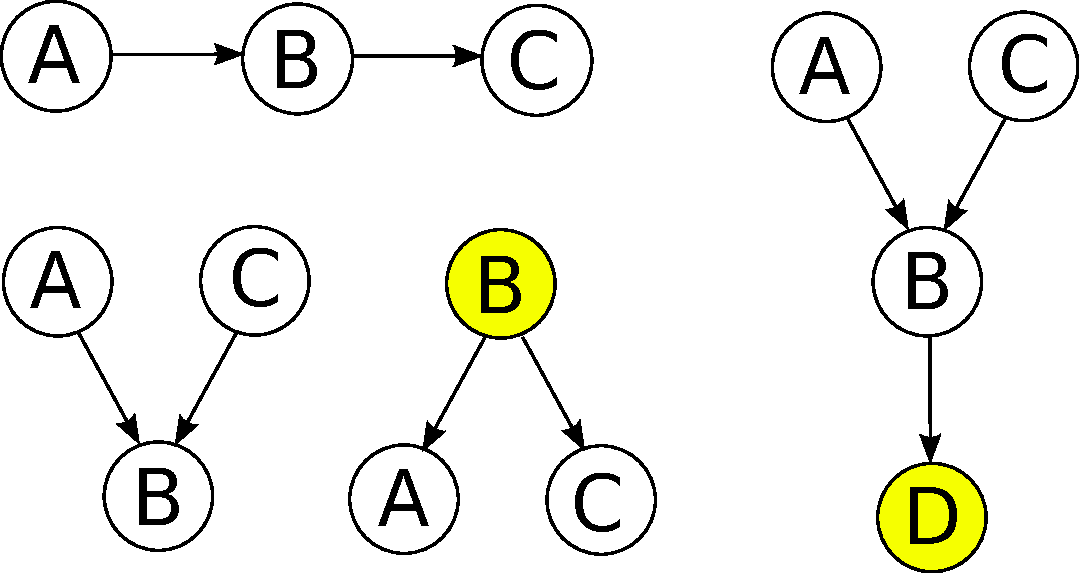
\includegraphics[height=0.3\textwidth]{ActiveTriplet.pdf}
\end{figure}

The events $A$ and $C$ are dependent on each other if they are connected in the Bayes network in the way shown on the image above. The yellow events are in the defined state (they are given, known), while the white events are in the undefined state.


\paragraph*{Independent events in the Bayes networks}

\begin{figure}[h!]
\centering
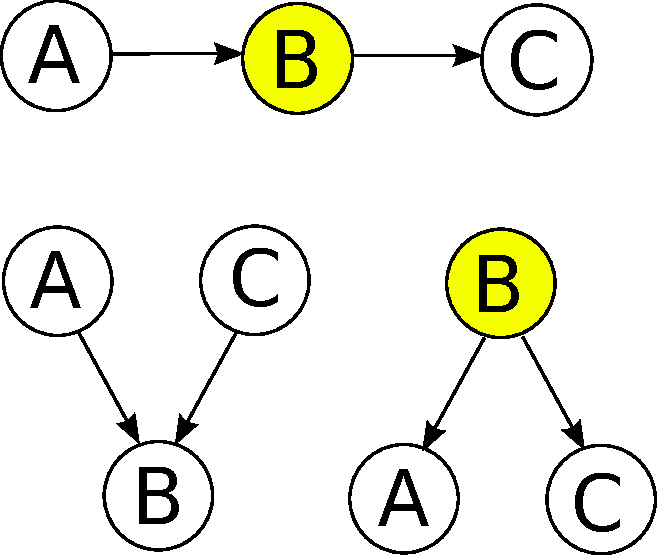
\includegraphics[height=0.3\textwidth]{InactiveTriplet.pdf}
\end{figure}

The events $A$ and $C$ are independent on each other if they are connected in the Bayes network in the way shown on the image above.

\subsection{Gaussian distribution}

Gaussian distribution (normal distribution) is a \textbf{continuous probability distribution} that is often used as a first approximation to describe real-valued random variables that tend to cluster around a single mean value $\mu$ with the variance $\sigma^2$.

\begin{figure}[h!]
\centering
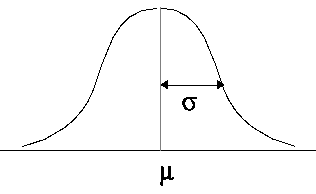
\includegraphics[height=0.25\textwidth]{Gaussian.png}
\end{figure}
Gaussian distribution is mathematically described by the function:
\[ f(x) = \frac{1}{\sqrt{2 \pi }\sigma} \exp \left(- \frac{1}{2} \frac{(x-\mu)^2}{\sigma^2} \right) \]
The integral of Gaussian function is 0, and it's maximum is at $x=\mu$.

\paragraph{Multivariate Gaussian}
In the $N$-dimensional space the multivariate Gaussian distribution is used, given by the formula:
\[ f(x) = (2 \pi)^{-\frac{N}{2}}) | \Sigma |^{\frac{1}{2}} \exp \left(- \frac{1}{2} (x-\mu)^T \Sigma^{-1} (x-\mu) \right) \]
where $\Sigma$ is the covariance matrix.

\part*{Machine learning}

Machine learning is the major area of artificial intelligence.

In machine learning we try to learn models, \textbf{structure}, \textbf{parameters} and \textbf{hidden concepts} from available data. We may use different target information. In \textbf{supervised learning} we use specific target labels, in \textbf{unsupervised learning} the target labels are missing and we use replacement principles and in \textbf{reinforced learning} the agent learn from the feedback from the environment. 

With machine learning we can make \textbf{predictions}, \textbf{diagnose}, \textbf{summarize}. The learning may be \textbf{passive}, when the agent does not impact the data or \textbf{active} where id does influence it. It may occur \textbf{on-line}, while the data is being generated or \textbf{off-line}, on the data already generated.

The output may be binary or is having the fixed number of classes (\textbf{classification}) or continuous (\textbf{regression}). \textbf{Generative} machine learning methods try to model the data as generally as possible and \textbf{discriminative} methods seek to distinguish data.

\section{Supervised machine learning}

In the supervised learning in each training example the \textbf{feature vector} and the \textbf{target label} are given. Basing on the training examples we wish to produce an fiction that predicts the target label basing on feature vector.

The data (feature vectors $x_m=(x_{m1}, x_{m2}, ... x_{mn})$ and target labels $y_m$) may be denoted:
\[
\left[ \begin{array}{ccccccc}
x_{11} & x_{12} & x_{13} & \cdots & x_{1n} & \rightarrow & y_1 \\
x_{21} & x_{22} & x_{23} & \cdots & x_{2n} & \rightarrow & y_2  \\
	&      & \vdots &      &      &             &      \\
x_{m1} & x_{m2} & x_{m3} & \cdots & x_{mn} & \rightarrow & y_m \end{array} \right]
\]
The function we seek basing on data is denoted $f(x_m)=y_m$. The certain amount of error in training data is usually tolerated. Then we use this function to make predictions $f(x)=y$.

We talk about \textbf{classification} problem if the target label is discrete. Problems where the target label is continuous are called \textbf{regression} problems. In regression problems we can't use the Bayes networks, because they can't handle continuous values.

The supervised learning methods can be divided into \textbf{parametric} and \textbf{non-parametric} methods. In parametric methods the number of parameters that algorithm have to figure out is independent of the training set size. Parametric methods include Naive Bayes and linear regression. In non-parametric methods the number of parameters can grow over time.

\subsection{Occam Razor}
\begin{center}\textit{If everything is being equal, choose the less complex hypothesis.}\end{center}
Usually we can fit the data with many functions and we always have the trade-off between data fit and low complexity. The more complex the hypothesis, the smaller the \textbf{training data error}, but the \textbf{over-fitting error} tends to get bigger. The sum of the training data error and over-fitting error is called \textbf{generalization} error and should be minimized to get the best fit. Over-fitting is the major source of the poor performance of the AI algorithms. 
\vspace{1em}

\begin{center}
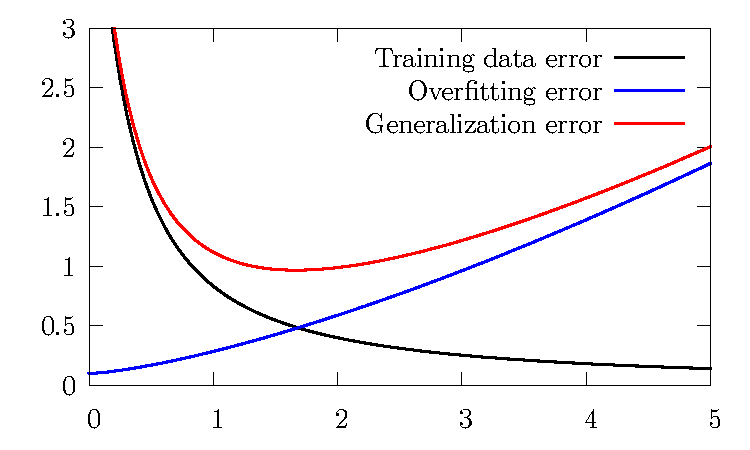
\includegraphics[width=0.7\textwidth]{OccamRazor.pdf}
\end{center}

\subsection{Classification}

\subsubsection{Spam detection by Naive Bayes}

In spam detection target label is mail being either spam or ham, and feature vector is an email content. Text document can be represented as \textbf{bag of words} - the dictionary of words with their number of occurrences in the text.

We can construct a Bayes network representing spam detection problem as shown below. The node $Y$ represents the target label variable and the children nodes $X_n$ representing elements of feature vector (here words from bag of words) and their conditional probability of occurrence for given value of $Y$. The goal of algorithm is to find the parameters in given Bays network basing on test examples.

\begin{center}
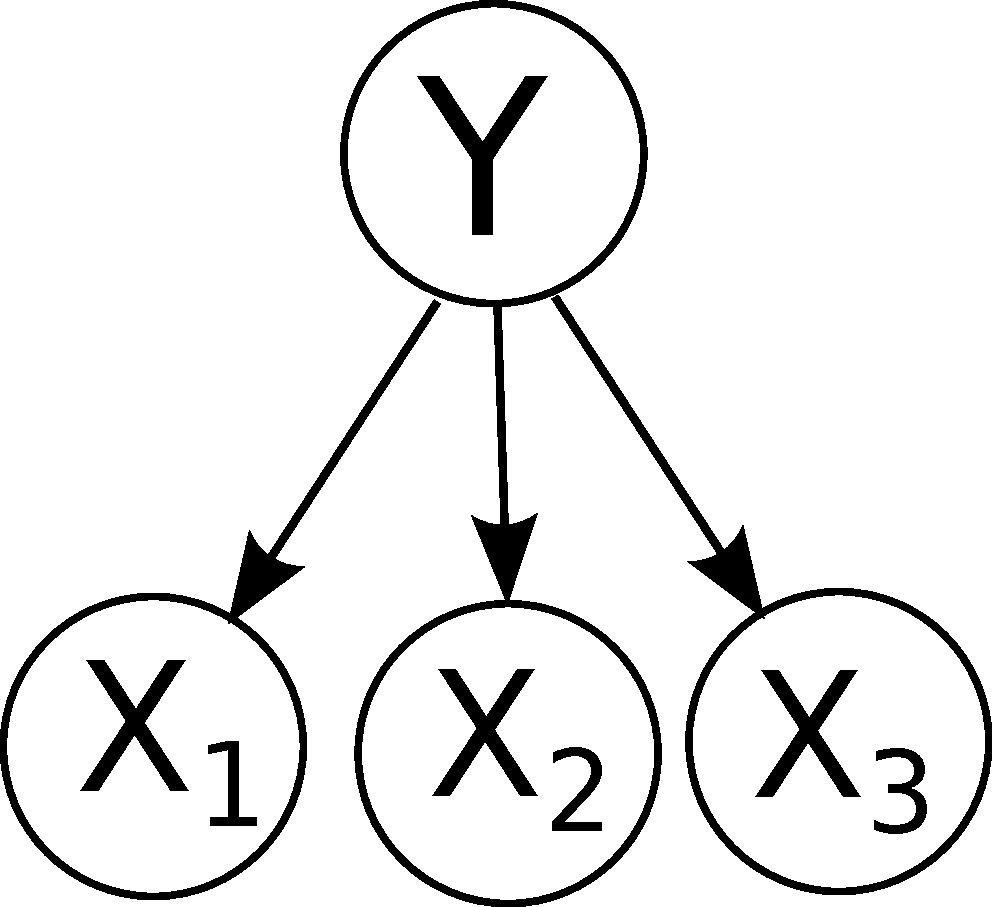
\includegraphics[width=0.2\textwidth]{NaiveBayes.pdf}
\end{center}

In this simple method the probability that message $M$ consisting of words $M_1$, $M_2$, ... $M_n$ is a spam is given by the expression:
\[ p(spam|M) = \frac{p(M|spam)p(spam)}{p(M)} = \frac{p(M|spam)p(spam)}{p(M|spam)p(spam) + p(M|ham)p(ham)} = \]
\[ = \frac{p(M_1|spam)\cdot ...\cdot p(M_n|spam)p(spam)}{p(M_1|spam)\cdot ...\cdot p(M_n|spam)p(spam) + p(M_1|ham)\cdot ...\cdot p(M_n|ham)p(ham)}  \]
The probabilities in this expression can be estimated basing on training data in different ways.

\paragraph*{Maximum likelihood}

In the maximum likelihood method we estimate the probability of the variable x having the given value in the simple way, that is:
\[p(x) = \frac{\mathrm{count}(x)}{N} \]
The maximum likelihood tends to over-fit the training data - if the message M contains a single word which did not occur in the training examples of spam messages, the probability of this message being spam is calculated as 0.

\paragraph*{Laplace smoothing}

In Laplace smoothing method we use a different way to estimate probability of variable x having given value. We introduce an additional parameter $k$:
\[ p(x) = \frac{\mathrm{count}(x)+k}{N+k\cdot |x|} \]
The variables used in this mathematical descriptions are:
\begin{itemize}
\setlength{\itemsep}{0pt}
\setlength{\parskip}{0pt}
\setlength{\parsep}{0pt}
\item $x$ is a variable
\item $|x|$ is the number of values that the variable x can take on
\item count($x$) is the number of occurrences of specific value of the variable x
\item $N$ is the total number of occurrences of x (the variable, not the value) in the sample size
\end{itemize}

\paragraph*{Cross validation}

It is a method to avoid over-fitting and find a good parameter k in the Laplace smoothing. It needs a big set of training data to work correctly.

The set of training data is divided into three subsets: "train" set ($~$80\%), "cross-validate" set ($~$10\%) and "test" set ($~$10\%). The train set is used to find all the parameters of Bayes network. It is done for the different values of $k$ and then the cross-validate set is used to determine which value of $k$ maximizes the efficiency of the algorithm. At the end the performance is (only once) validated on test set of training data.

\subsubsection{Perception algorithms}
\paragraph{Linear separation}

This is an algorithm to find a \textbf{linear separator} between the two sets of data, as shown on the picture. It only converges if data is linearly separable.

\begin{center}
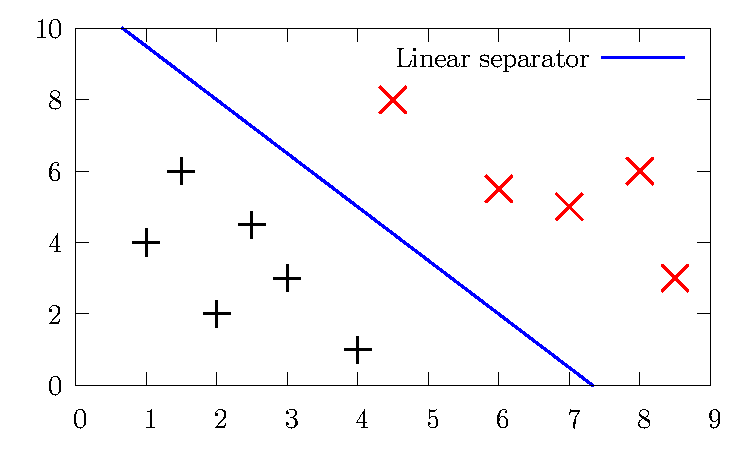
\includegraphics[width=0.7\textwidth]{PerceptionAlgorithm.pdf}
\end{center}

The linear separation classification function is:
\[
  f(x) = \left\{ 
  \begin{array}{l l l}
    1 & \mathrm{if} & w_1 x + w_0 \geq 0\\
    0 & \mathrm{if} & w_1 x + w_0 < 0\\
  \end{array} \right.
\]
To start the algorithm we randomly choose values for $w_0$ and $w_1$ and then calculate the followinf iteration steps:
\[ w_i^{m+1} = w_i^m + \alpha (y_j - f(x_j) ) \]
$\alpha$ is a small \textbf{learning rate} and parenthesis $(y_j - f(x_j))$ are the error for the $j$ data point. Thus only where the point is not given the right label by the function $f(x)$, the update occurs and the update is proportional to the size of the error.

\paragraph{k-Nearest neighbours}

In this algorithm for separation in the learning process memorizes all the test vectors and their labels. Then given the new example it finds the k nearest neighbours from the training set and chooses for the new example the label that majority of the neighbours is having.

The value of k is a \textbf{regularizer}. The higher the k, the smoother the separation boundaries are becoming. The cross-validation can be used to choose value of k.

For the very large data sets the k-Nearest neighbours algorithm is slow, because it searches a big dataset to find the neighbours. The solution may be to represent the data as a tree.

The very large feature spaces also causes the problems, because most of the neighbours are really far away from each other. Thus the k-Nearest neighbours works good only for small feature spaces, having up to 4 dimensions.


\subsection{Regression}
\subsubsection{Linear regression}

In linear regression the function $f(x)=y$ we look for basing on training set consisting of feature vectors $x_m=(x_{m1}, x_{m2}, ... x_{mn})$ and target labels $y_m$ is having a specific form:
\[ f(x) = w_1x+w_0\]

The goal of the linear regression is to minimize the \textbf{loss function} describing the residual error after fitting the data as good as possible. In can be described by quadratic error:
\[\mathrm{LOSS} = \sum_{j} \left( y_j - w_1 x_j - w_0\right)^2\]
The $j$ enumerates all the training examples. The optimal set of parameters $w^*$ can be described as
\[w^* = \min_w \mathrm{LOSS} = \min_w \sum_{j} \left( y_j - w_1 x_j - w_0\right)^2 \]
This minimization can be solved explicitly giving the answer:
\[ w_1^* = \frac{M \sum x_i y_i - \sum x_i \sum y_i}{M \sum x_i^2 - \left( \sum x_i \right)^2 } \]
\[ w_0^* = \frac{1}{M} \sum  y_i - \frac{w_1}{M}\sum x_i \]

The drawbacks of the linear regression are:\begin{itemize}
\item it is suitable only for linear data,
\item one training data point being very far from linearity (while all the other points are more or less on the line) tends to spoil the outcome
\item for value of $x$ going to infinity $y$ also goes to infinity, which is sometimes undesirable.
\end{itemize}

\subsubsection{Logistic regression}

In logistic regression the problem of $y$ going to infinity with growing $x$ is addressed. The function we fit is:
\[ g(x) = \frac{1}{1+e^{-f(x)}} \]
where $f(x)$ is a linear function. 
\[g(x) \in (0,1)\]

\subsubsection{Regularization (complexity control)}

The LOSS function can be modified to include the complexity control term, depending of parameters, penalize the parameters for growing large.

\[\mathrm{LOSS} = \mathrm{LOSS}(data) + \mathrm{LOSS}(parameters) = \]
\[ = \sum_{j} \left( y_j - w_1 x_j - w_0\right)^2 + \sum_i (w_i)^p \; \; \; \; \; p \in {1,2} \]

\subsubsection{Gradient descent}

Minimizing the loss functions more complicated than for linear regression usually does not have the closed form solution. We need to use the other methods, such as iteration methods.

In this method we start with initial guess of $w^0$. Then we compute the next approximations from the formula
\[w^{i+1} = w^i - \alpha \nabla_{w} L(w^i) \] 
The drawback of the gradient descent method is that it may find only the local minimum of the function, not the global minimum.

\section{Unsupervised learning}

In the unsupervised learning the agent is given the data matrix consisting of \textbf{M data items} of \textbf{N features} each. However, no target labels are given, unlike in supervised learning. The task for the unsupervised learning is to find a structure of the data of this type.

\[
\left[ \begin{array}{ccccc}
x_{11} & x_{12} & x_{13} & \cdots & x_{1n}  \\
x_{21} & x_{22} & x_{23} & \cdots & x_{2n}  \\
	&      & \vdots &      &      \\
x_{m1} & x_{m2} & x_{m3} & \cdots & x_{mn} \end{array} \right]
\]
\subsection{Gaussian learning}
The problem we want to solve is what is the Gaussian function best fitting the given data. The parameters of Gaussian function are mean $\mu$ and variance $\sigma^2$ in one-dimensional case.

\[ f(x|\mu, \sigma^2) = \frac{1}{\sqrt{2 \pi \sigma^2 }} \exp \left(-\frac{(x-\mu)^2}{2 \sigma^2} \right) \]

To fit Gaussian function to the data we take $\mu$ as the average of data and $\sigma^2$ as the average quadratic deviation of the data:
\[ \mu = \frac{1}{M} \sum_{j=1}^M x_j \]
\[ \sigma^2 = \frac{1}{M} \sum_{j=1}^M (x_j - \mu)^2 \]

\subsection{Density estimation}

I the data is independent and identically distributed \textbf{iid}, which means each random variable has the same probability distribution as the others and all are mutually independent, we can try to recover the density of probability distribution that generated the data.

Methods used for this task include \textbf{clustering} and \textbf{dimensionality reduction}.

\subsubsection{Clustering}

\paragraph{k-means}

This method estimates, for the fixed number of k, the k best centres of clusters representing given data points. The algorithm is iterative:

\begin{verbatim}
initially: select k cluster centres of random
  repeat
    correspond the data points to nearest clusters
    update the cluster center by mean of corresponding data points
    empty cluster centres: restart of random
  until
    no change
\end{verbatim}

The problems with k-means algorithm include the need to know the number of clusters we look for, the danger of finding the local minima by the algorithm instead of global minima, the problem of calculating distances for the high-dimensional problem and the lack of the mathematical basis of the algorithm. The advantage is that the algorithm is easy to implement.

\paragraph{Expectation maximization}

This algorithm is the generalization of k-means algorithm.

%TODO

\section{Representation with logic}

\subsection{Prepositional logic}	

In prepositional logic the state of each variable is either true, false or unknown. 
We use the logical symbols to construct the sentences:
\begin{itemize}
\setlength{\itemsep}{0pt}
\setlength{\parskip}{0pt}
\setlength{\parsep}{0pt}
\item $\vee$ logical disjunction (or)
\item $\wedge$ logical conjunction (and)
\item $\Rightarrow$ implication (if ... then)
\item $\Leftrightarrow$ equivalence (if and only if)
\item $\lnot$ negation (not)
\end{itemize}
Each prepositional logic sentence is true or false with respect to the model of the world. The model is the set of true-false valued of all the prepositional symbols. We can evaluate the truth of the sentence depending of truth ow the words using \textbf{truth tables}.

\begin{displaymath}
\begin{array}{|c|c||c|c|c|c|c|}
\hline
   P & Q & \lnot{}P & P\land{}Q & P\lor{}Q & P\Rightarrow{}Q & P\Leftrightarrow{}Q \\
\hline
false & false & true & false & false & true & true \\
false & true & true & false & true & true & false \\
true & false & false & false & true & false & false \\
true & true & false & true & true & true & true \\
\hline
\end{array}
\end{displaymath}

\textbf{Valid sentence} is a sentence true in every possible model - for every possible combination of values of propositional symbols. \textbf{Satisfiable sentence} is one that is true in some model but not necessarily all of the models. \textbf{Unsatisfiable sentence} is the one which is false for all the models.

Limitations of propositional logic:\begin{itemize}
\setlength{\itemsep}{0pt}
\setlength{\parskip}{0pt}
\setlength{\parsep}{0pt}
\item It is unable to handle uncertainty
\item It can talk only about events that are true or false. It can't talk about objects, their properties and relations between them.
\item There are no short-cuts. 
\end{itemize}

\subsection{First order logic}

It is the extension of prepositional logic which can describe relations, objects and their functions.  Each of those can be either true, false or unknown.

The model in first order logic consists of the set of \textbf{objects}, set of \textbf{constants} that refer to those objects (but it does not have to be one-to-one correspondence between constants and the objects) and the set of \textbf{functions}, which are defined as mappings from objects to objects. There are also \textbf{relations}, defined on one, many or no object at all.

In first order logic here are \textbf{sentences} describing facts and \textbf{terms} describing objects. 

Terms can be constants, variables and functions. Sentences correspond to relations (and specifically to equality relations), and they can be combined by operators same as in perceptional logic: $\vee$ $\wedge$ $\Rightarrow$ $\Leftrightarrow$ $\lnot$. To construct sentences we can also use \textbf{quantifiers}:
\begin{itemize}
\setlength{\itemsep}{0pt}
\setlength{\parskip}{0pt}
\setlength{\parsep}{0pt}
\item $\forall$ for all
\item $\exists$ there exists
\end{itemize}

\subsubsection*{Vacuum world}

The example of world that can be described by first-order logic is an vacuum world.

\begin{figure}[h!]
\centering
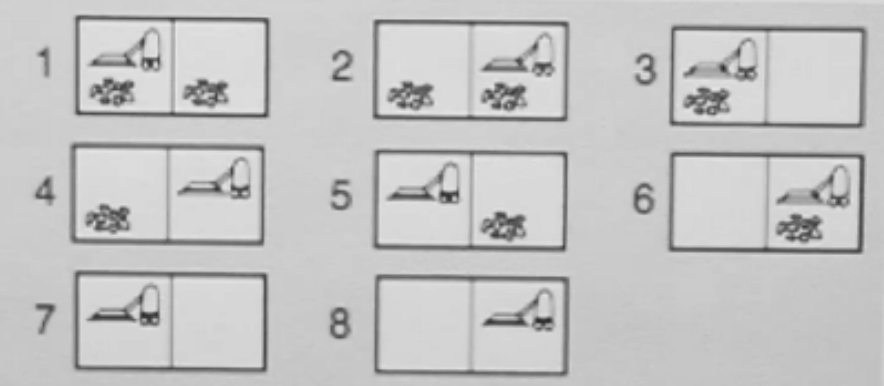
\includegraphics[height=0.3\textwidth]{vacuum_world.png}
\end{figure}

The \textbf{objects} in this world are locations $A$ and $B$, vacuum cleaner $V$ and two pieces of dirt $D_1$ and $D_2$. The \textbf{relations } are $Loc(x)$ (true for any location), $Vacuum(x)$ (true for any vacuum, $Dirt(x)$ (true for any dirt) and add $A+(x,y)$ which is true for an object and an location.

Examples of the sentences in the vacuum world are:
\begin{itemize}
\setlength{\itemsep}{0pt}
\setlength{\parskip}{0pt}
\setlength{\parsep}{0pt}
\item $A+(V,A)$ \\Vacuum is at location A.
\item $\forall_d \forall_l \; Dirt(d) \vee Loc(l) \Rightarrow \lnot A+(d,l)$ \\There is no dirt in any location.
\item $\exists_l \exists_d \; Dirt(d) \vee Loc(l) \vee A+(V,l) \vee A+(d,l) $ \\The vacuum is in the location with dirt.
\end{itemize}

\section{Planning}

The problem solving techniques work only if the environment is deterministic fully observable. Using planning techniques we can relax those constraints. In planning methods the given task is realized by agent using the constant feedback from the environment, so that during executing some plan this plan is constantly modified to fit better to the environment the agent interacts with.

If the environment is \textbf{stochastic} we can't know for sure what will be the result of our action, and we have to react accordingly to this effect. If the environment is \textbf{multiagent}  we have to react to the behaviour of the other agents which is known only at the execution time, not at the planning time. If the environment is \textbf{partially observable} we don't know from the beginning what is the state of the environment - we learn that only during the execution. In all those situations planning techniques are suitable.

To solve those problems we can plan in the space \textbf{belief states} instead of the space of real states.

\subsection{Belief states space}

Belief states space contains all states that agent can be in basing on the information available about partially-observable environment. Space of belief states changes when agent performs action or senses the environment - the states themselves can change as well as the dimensionality of the space.

In \textbf{deterministic environments} each action taken is having the one possible result, and thus action taken by agent can preserve or reduce the dimensionality of the belief states space. The dimensionality is reduced if actions starting from different states lead to the same state. Observation (sensing the environment) also can preserve dimensionality, if we don't learn anything new about the environment, or reduce it when new information is gained. In fact it partitions the belief states space.

In \textbf{stochastic environments} when agent takes action the dimensionality of belief states space increases, because the result of the action is not known - there may be many results with different possibilities of occurrence. On the other hand sensing environment can, as in deterministic environment, only preserve or reduce the dimensionality.

\end{document}